
\section{Events and Source Properties}

The 30 earthquakes considered for the evaluation of the models in this article are labeled with a sequential letter-code from A to to AD in Fig.~\ref{fig:region} with their detailed information presented in Table \ref{tab:events}  \citet{Lee_2011_GJI}.
They are a set of earthquakes which are happened between 1998 and 2014, and had magnitudes between 3.6 and 5.4, and hypocenter depths that vary between 3.6 and 21.1~km. Events are modeled as a point source analogy with rupture parameters scaled according to the magnitude of each earthquake and source time functions respecting to that.



\begin{table}
	\centering\small

	\caption{Information for 30 events including their ID \citet{SCEC}, magnitude and final number of stations.}
	\begin{tabular}{|c c c c || c c c c}
	
	\hline

	  	Code								& 
	  	Event ID							& 
	  	\eqmag{w}							&
	  	Num.								&
	  	Code								& 
	  	Event ID							& 
	  	\eqmag{w}							&
	  	Num.								\\
	\hline																																
		A			&	 9064568	&	4.40	&	17&  P&	14312160	&	4.66	&	109	\\ % A 

		B				&	10972299	&	3.79	&	52&	Q&	15237281	&	3.86	&	120\\ % R
		C				&	14494128	&	3.72	&	77&	R&	 9703873	&	4.24	&	130\\ % Z
		D					&	14155260	&	4.88	& 172&	S&	10410337	&	4.70	&	213\\ % V
																					
		E		&	10216101	&	3.60	&	55&	T&	 9716853	&	3.98	&	55\\ % J
																					
		F				&	13692644	&	3.74	&	55&	U&	 9093975	&	3.77	&	25\\ % S
		G				&	14116972	&	4.42	&	83&	V&	14601172	&	4.44	&	180\\ % U
		H			&	10370141	&	4.45	&	159 &	W&	15481673	&	5.10	&	311\\ % L
		I			&	 9140050	&	4.37	&	38&	X&	14383980	&	5.39	&	335\\ % D
		J					&	10541957	& 4.10&	97&	Y&	 9818433	&	4.75	&	67\\ % Q
		K				&	10530013	&	4.28	& 76	& Z&	10399889	&	3.98	&	91\\ % P
		L				&	14239184	&	3.90	&	66&	AA&	 9644101	&	3.64	&	53\\ % W
																					
		M				&	14000376	&	3.59	&	54&	AB&	10275733	&	4.73	&	116\\ % T
		N			&	 9753489	&	3.90	&	52&	AC&	10403777	&	4.42	&	94\\ % H
		O			&	 9096972	&	3.98	&	26&	AD&	14738436	&	3.69	&	93\\ % C
		\hline
																				
	\end{tabular}
	\label{tab:events}
\end{table}




\begin{figure}
    \centering
    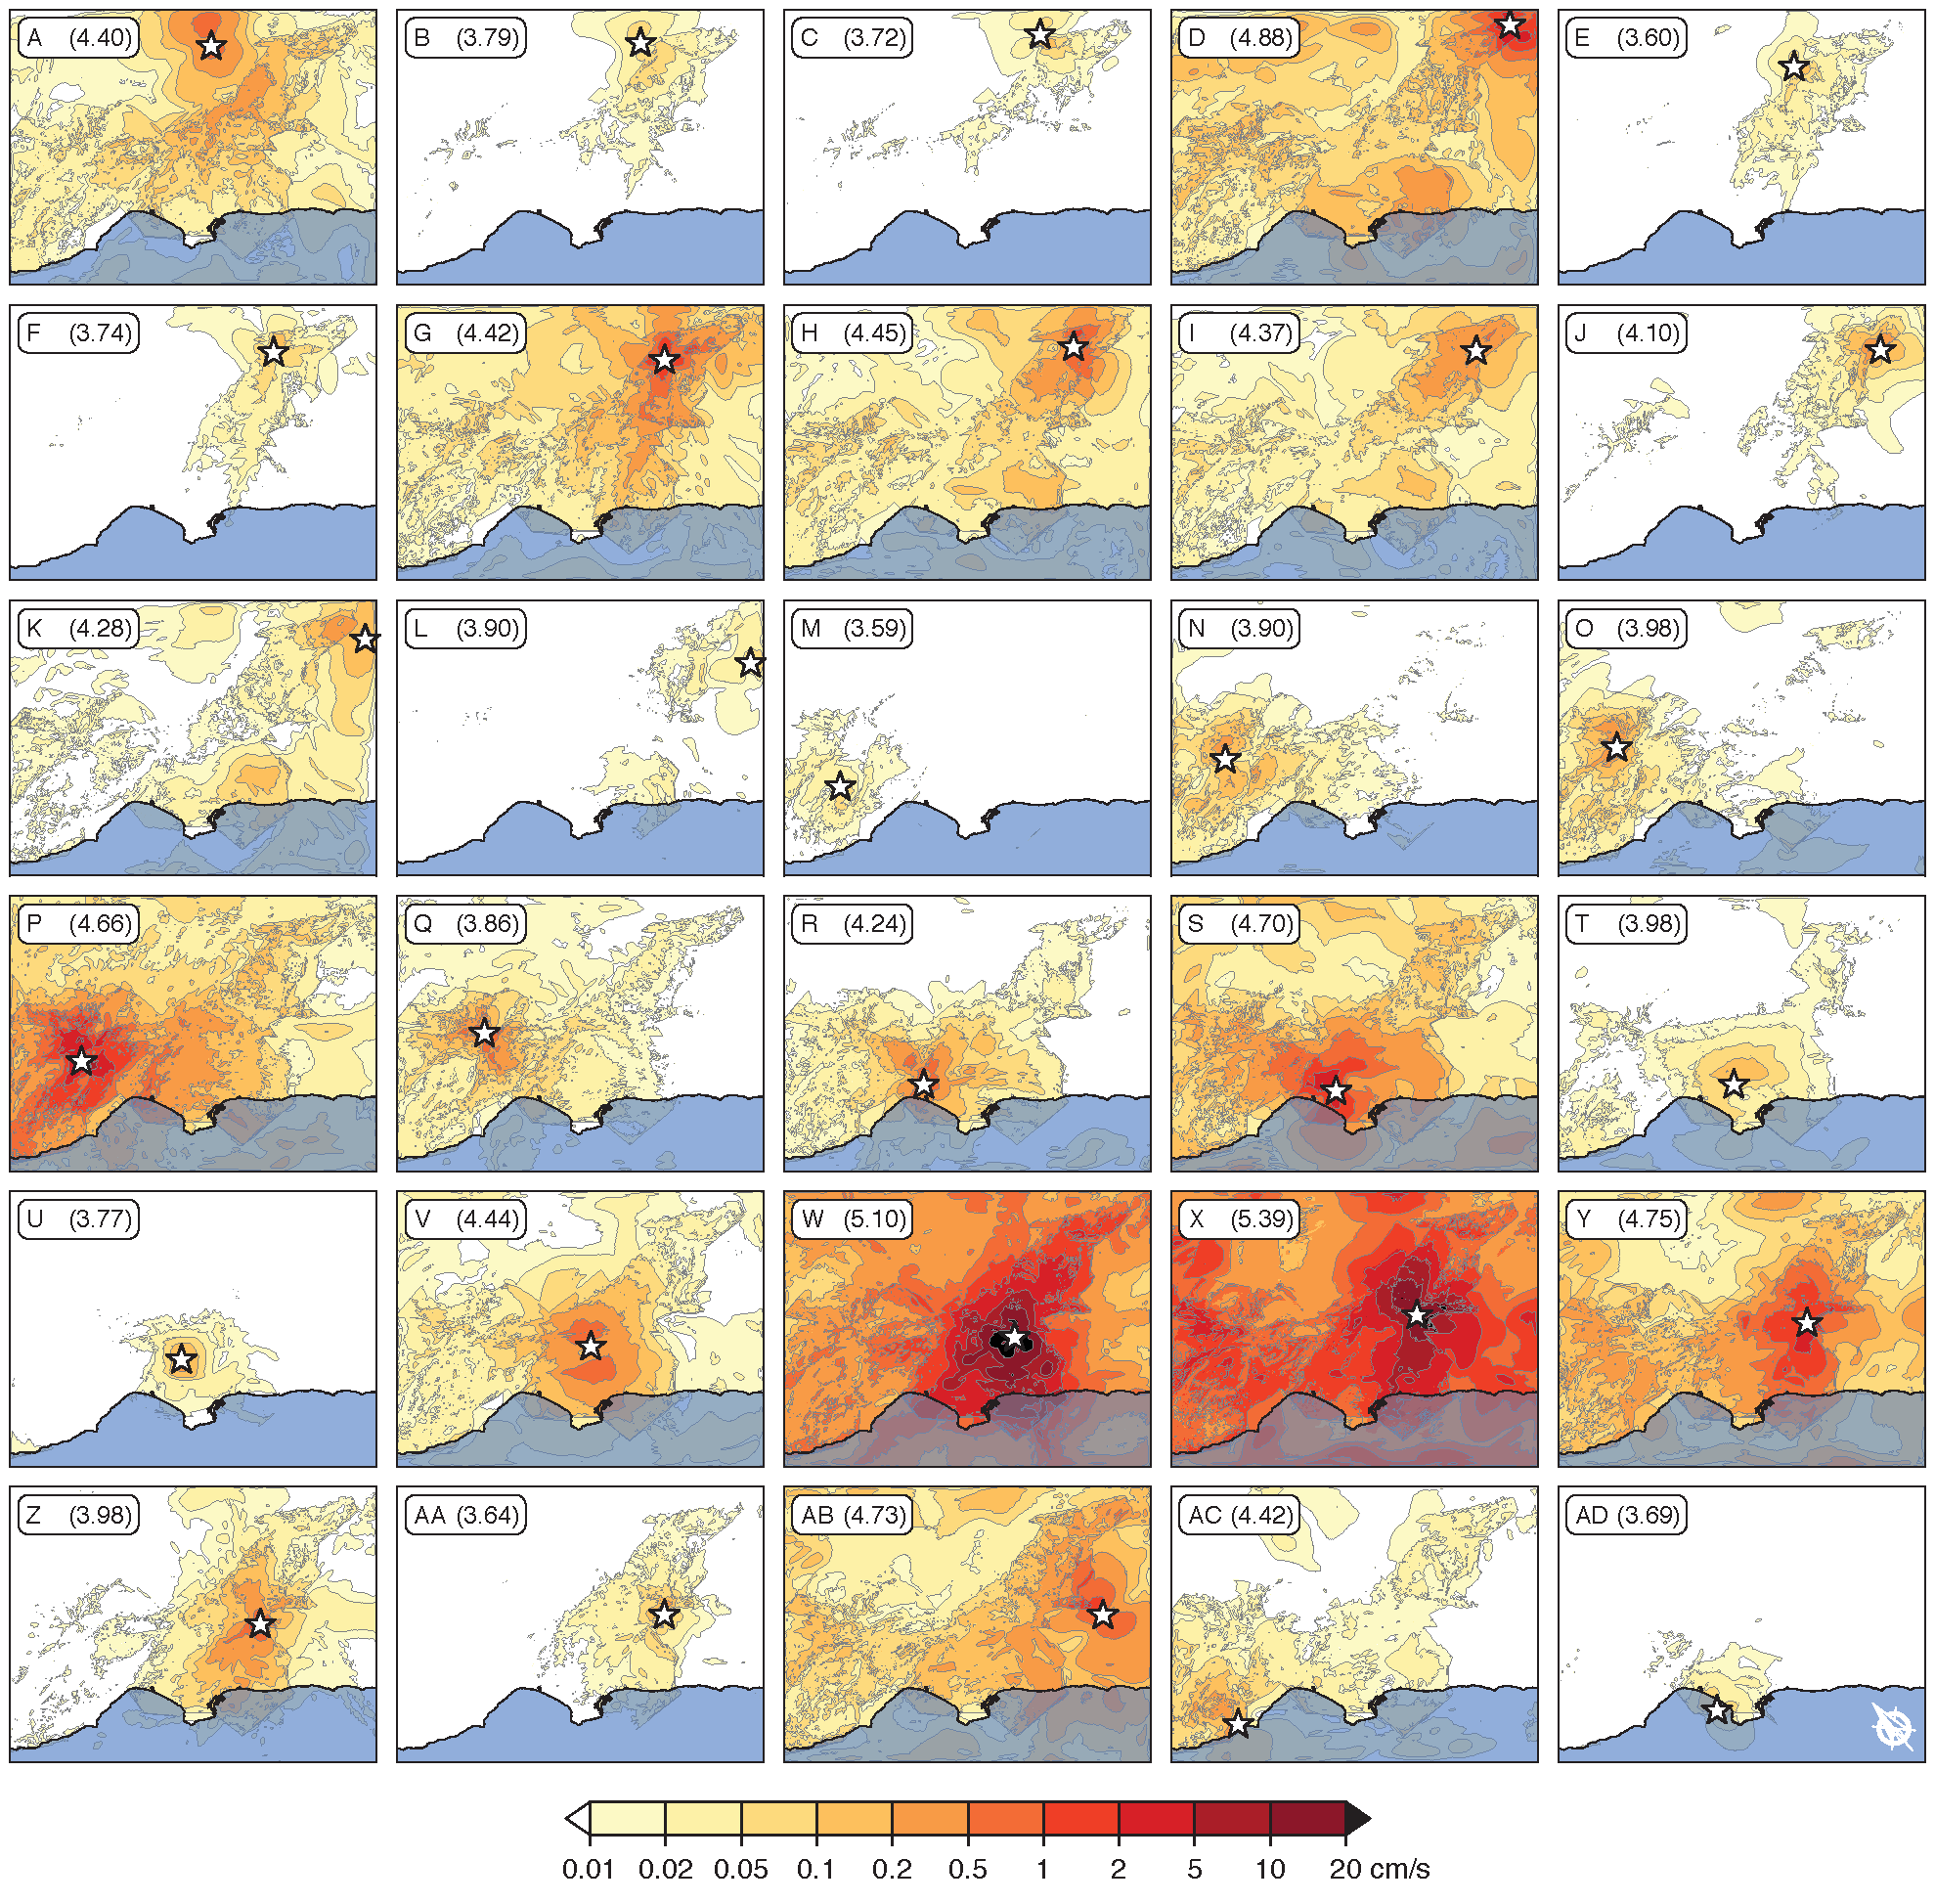
\includegraphics
        [width=\columnwidth]
        {figures/pdf/figure-03}
    \caption{Source time functions (top: slip; middle: slip-rate), and slip-rate Fourier amplitude spectra (bottom) of all the events. Slip-rate functions were computed based on the total rise time estimated from eqs~(\ref{eq:stein}) and (\ref{eq:sliprate}). The source functions of events W and X, corresponding to the 2014 La Habra and 2008 Chino Hills earthquakes, are singled out in the figure because for reference. These two events are the largest of all earthquakes considered.}
    \label{fig:slip}
\end{figure}


